
\documentclass[sigconf]{acmart}
\usepackage{tcolorbox}
\usepackage{xcolor}
\usepackage{colortbl}
\usepackage{graphicx}
\newtcolorbox{mybox}{top=1pt,bottom=1pt,left=1pt,right=1pt,colback = white,boxrule = 0.3mm,arc = 0mm}
\definecolor{mygray}{gray}{.9}
\def\BibTeX{{\rm B\kern-.05em{\sc i\kern-.025em b}\kern-.08em
    T\kern-.1667em\lower.7ex\hbox{E}\kern-.125emX}}


\AtBeginDocument{%
  \providecommand\BibTeX{{%
    \normalfont B\kern-0.5em{\scshape i\kern-0.25em b}\kern-0.8em\TeX}}}


\setcopyright{acmcopyright}
\copyrightyear{2018}
\acmYear{2018}
\acmDOI{10.1145/1122445.1122456}


\acmConference[Internetware '20]{Woodstock '18: ACM Symposium on Neural
  Gaze Detection}{NOV 01--03, 2020}{Singapore}
\acmBooktitle{Woodstock '18: ACM Symposium on Neural Gaze Detection,
  June 03--05, 2018, Woodstock, NY}
\acmPrice{15.00}
\acmISBN{978-1-4503-XXXX-X/18/06}



\begin{document}


\title{An introduction to Docker Image Dependency Network: Structure, Diversity, and Link Paradigm}


\orcid{1234-5678-9012}
\author{G.K.M. Tobin}
\authornotemark[1]
\email{webmaster@marysville-ohio.com}
\affiliation{%
  \institution{Institute for Clarity in Documentation}
  \streetaddress{P.O. Box 1212}
  \city{Dublin}
  \state{Ohio}
  \postcode{43017-6221}
}

\author{Lars Th{\o}rv{\"a}ld}
\affiliation{%
  \institution{The Th{\o}rv{\"a}ld Group}
  \streetaddress{1 Th{\o}rv{\"a}ld Circle}
  \city{Hekla}
  \country{Iceland}}
\email{larst@affiliation.org}

\author{Valerie B\'eranger}
\affiliation{%
  \institution{Inria Paris-Rocquencourt}
  \city{Rocquencourt}
  \country{France}
}

\author{Aparna Patel}
\affiliation{%
 \institution{Rajiv Gandhi University}
 \streetaddress{Rono-Hills}
 \city{Doimukh}
 \state{Arunachal Pradesh}
 \country{India}}

\author{Huifen Chan}
\affiliation{%
  \institution{Tsinghua University}
  \streetaddress{30 Shuangqing Rd}
  \city{Haidian Qu}
  \state{Beijing Shi}
  \country{China}}

\author{Charles Palmer}
\affiliation{%
  \institution{Palmer Research Laboratories}
  \streetaddress{8600 Datapoint Drive}
  \city{San Antonio}
  \state{Texas}
  \postcode{78229}}
\email{cpalmer@prl.com}



\renewcommand{\shortauthors}{Trovato and Tobin, et al.}


\begin{abstract}
Docker images are not developed isolated. Instruction parameters inside dockfiles executing docker images generation links the docker images strongly. Prior studies have shown that docker images promote.......However, these studies did not explore the interconnection and development between images.

In this paper, we contibute to a method of constructing dependency network of docker images from a large-scale dockerfiles. We find that most dockr images are centered around one image and furthermore identify these influential images. We establish the sub-network of influential images and analyse their network structre. The most influencial docker images characters as Operating system and Programing language pushed the develpoment of software development together. We furthermore explore the inner causes of interconnected sub-networks and find that the interconnected closely sub-networks contribute to development of software.
\end{abstract}


\begin{CCSXML}
<ccs2012>
 <concept>
  <concept_id>10010520.10010553.10010562</concept_id>
  <concept_desc>Computer systems organization~Embedded systems</concept_desc>
  <concept_significance>500</concept_significance>
 </concept>
 <concept>
  <concept_id>10010520.10010575.10010755</concept_id>
  <concept_desc>Computer systems organization~Redundancy</concept_desc>
  <concept_significance>300</concept_significance>
 </concept>
 <concept>
  <concept_id>10010520.10010553.10010554</concept_id>
  <concept_desc>Computer systems organization~Robotics</concept_desc>
  <concept_significance>100</concept_significance>
 </concept>
 <concept>
  <concept_id>10003033.10003083.10003095</concept_id>
  <concept_desc>Networks~Network reliability</concept_desc>
  <concept_significance>100</concept_significance>
 </concept>
</ccs2012>
\end{CCSXML}

\ccsdesc[500]{Software and its engineering~Software development techniques}
\ccsdesc[300]{Computer systems organization~Redundancy}
\ccsdesc{Computer systems organization~Robotics}
\ccsdesc[100]{Networks~Network reliability}


\keywords{image dependency network, structre, diversity, revelence}



\maketitle

\section{Introduction}
With the popularity of DevOps driven by real efficiency in developing software system, an increasing amount of attention is being placed on Container, such as Docker charactering as lightweight virtualization technology to deploy software infrastructure. Docker images defined by Dockerfile's declarative instructions package an application with its dependencies execution environment and function as running Docker Contaier.

As software system grows in scale and complexity,so does Docker. The research on growth of docker images whose content defined completely by dockerfile can be done through the research of prasing dockerfiles. Mining potential link or knowledge of docker images with their scale expanding regularly would be valuable. Previous studies focuxes on optimization of docker configuration or the fast and high quality build of dockerfiles, however, rarely mentioned the realitionship and knowledge between docker images.......
 
Given the ubiquitous nature in industry, we study the inter connection between docker images, especially those core images brought strong appeal and cohesion. The "FROM" instruction defined by docker rule decide the reliable realitionships between a pair of docker image. Furturemore, docker images mostly built from other base image can also function as other directed base image which depends the interconnetd realitionships between docker images. Based on the above ubiquitous realitionships nature, we gain the strong dependency realitionships and future explore the dependency character through network mertics. 

We conduct an exploratory empirical study with the goal of charactering the dependency network between docker images and capturing the interconnected realitionships and analysing the inter connection causes between sub-networks centraled by influencial images.
 
In summary,we make three core contributions through our exploratory study:
The highlights of our quantitative findings are:

\begin{itemize}
\item \textbf{We conduct the first large-scale empirical study to construct and analyse dependency realitionships between docker images by network structre metric.}
\item \textbf{We find the TOP-100 influential images and explore the character of the sub-networks constructed by these images}
\item \textbf{We analyse the internal mechanism of sub-network development and future analyse the inter causes hiddend dockerfile resulting the interactive links between sub-network.}
\end{itemize}

Our data and source codes are online at





%\section{records}
%and we highlight some key future research directions to improve the Ethereum ecosystem.

 %fundamental data analysis task

%Overview and Analysis of Docker Image Dependency Network: Structure, Diversity, and Link Paradigm


\section{Research Setup}
Figure 1 gives the overview of our study. Based on the RQs, we perform quantitative studies ...

\subsection{Construct Image Dependency Network}
The instructions stored in Dockerfile define naturally the content of docker images, including the application, dependencies along with the execution environment. Especially, a valid Dockerfile must start with a  \emph{FROM instruction} where one docker image inherites infrastructure definitions from another image. The pointing realitionships captured by \emph{FROM instruction} can be regarded as technical dependency between Docker images. Specifically, we call image that have \emph{FROM instruction} pointing to other image \emph{linked},or \emph{source image}, and image that are linked to from other image's \emph{FROM instruction} \emph{linked to},or \emph{target image.} We say that a pair of images, I$_i$ from node i, and I$_j$ from node j, are a \emph{linked pair}, or \emph{link}, \emph{(I$_i$, I$_j$)}, if the \emph{FROM instruction} of node i point to node j. Indications of which target image the source image point upon can be obtained from the \emph{FROM instruction} used in the Dockerfiles.

To answer our research question, we construct the intergal image dependency network based on the technical dependency mentioned above. The \emph{Image Dependency Network} defined as a directed network \emph{N$_d$} = $\left \langle V,E \right \rangle$. The set of vertices, denoted by \emph{V}, is all docker images involved in at least one instruction link. The set of vertices, denoted by \emph{E}, is a set of node pairs \emph{E(V)} = $\left\{ 	\left( Ii, Ij \right)|Ii,Ij \in E. \right\}$ If the image represend by node x$_i$ instruction link the image represend by node y$_j$. The weight of each edge is the count of instruction link for the pair of docker images.\\




\subsection{Dataset}


%To enable our research, we remove the low-quality dockerfile including lake of FROM instruction, the value of FROM instruction parameter being null. Because of the several FROM instruction in one dockerfile, we capure all of them and resultly gain all the images pairs. After this filtering, we obtained our final set of 128,384 directed pairs of images.

%We first see the images with different versions have almost similar function and futher ignore the image tag to reveal more actural dependency realitionships.(e.g.. ubuntu and ubuntu3.6) We then remove  owner of images based on the hypothesis that different private owner create images with the same name to play a similar role in real usage environment.




We obtain all 129,463 dockerfiles in the form of folder from the public Github as the initial set. The producre of capturing Image Pairs form these dockerfiles showed as fig1.    %129,463

\noindent\textbf{Step1: Empty-Instruction Dockerfiles filtering} The Dockerfiles with empty \emph{FROM instruction} that provide infrastructure for building were first removed. As the study of yiwen Wu etc points out that dockerfile lacking of infrastructure can be considered as a low-quality build script, which is always prone to build failure in practice. To filter the empty instruction dockerfiles, we determine whether there are  \emph{FROM instruction} by parsing each dockerfile and got 128,247 available dockerfiles. After preliminary filtration of empty-instruction dockerfiles, we obtained 128,247 available dockerfiles.      %128,247  

\noindent\textbf{Step2: Obtaining Source Images} Dockerfiles are stored as folders, with the catalog information being owner/repository/Dockerfile. Thus, we remove the owner describing Image creator personal information and capture repository information/content identified as the Source Image id.   


\noindent\textbf{Step3: Obtaining Target Images}  This step can be divided into two sub processes: Firstly, \noindent\textbf{Geting available parsing parameters:} This process aims at prasing and capturing available parameters content by ingoring the \emph{FROM instruction} following with "\#" used for interpretative statement and filtering parameters containing variable eg..{base} having no specific meaning. After capturing available parameters and filtering useless content, we capture 130,830 target images id.
Afterwords, \noindent\textbf{Removing version information:} The content available of parameters in the following format as  base:version, base represents specific function while version changes without changing the basic functionality(e.g.. ubuntu and ubuntu3.6). Thus, we remove the version information anf future identify base as the Target Image id. % 130,830


\noindent\textbf{Step4: Combinating Image pairs} The obtained source image and target image, representing real identity information, have the consistent format. Further, we combine source image and target image corresponding to the same file as a Image pair in the form of (source image, target image). Resultly, we gor 130,830 image pairs. 
% 130,830

\noindent\textbf{Step5: Filtering Self reference Image pairs} Among 130,830 image pairs charactering techencial dependency relationship between images, there exist that source image is the same as the target image due to the remove of version. We consider this self reference image pair to be an invalid technical dependency and after this filter, We obtained 124,384 pairs of images pairs with effective technology dependence. %124384-1=124383     83030 nodes  

 
\begin{figure}[htbp]
\centerline{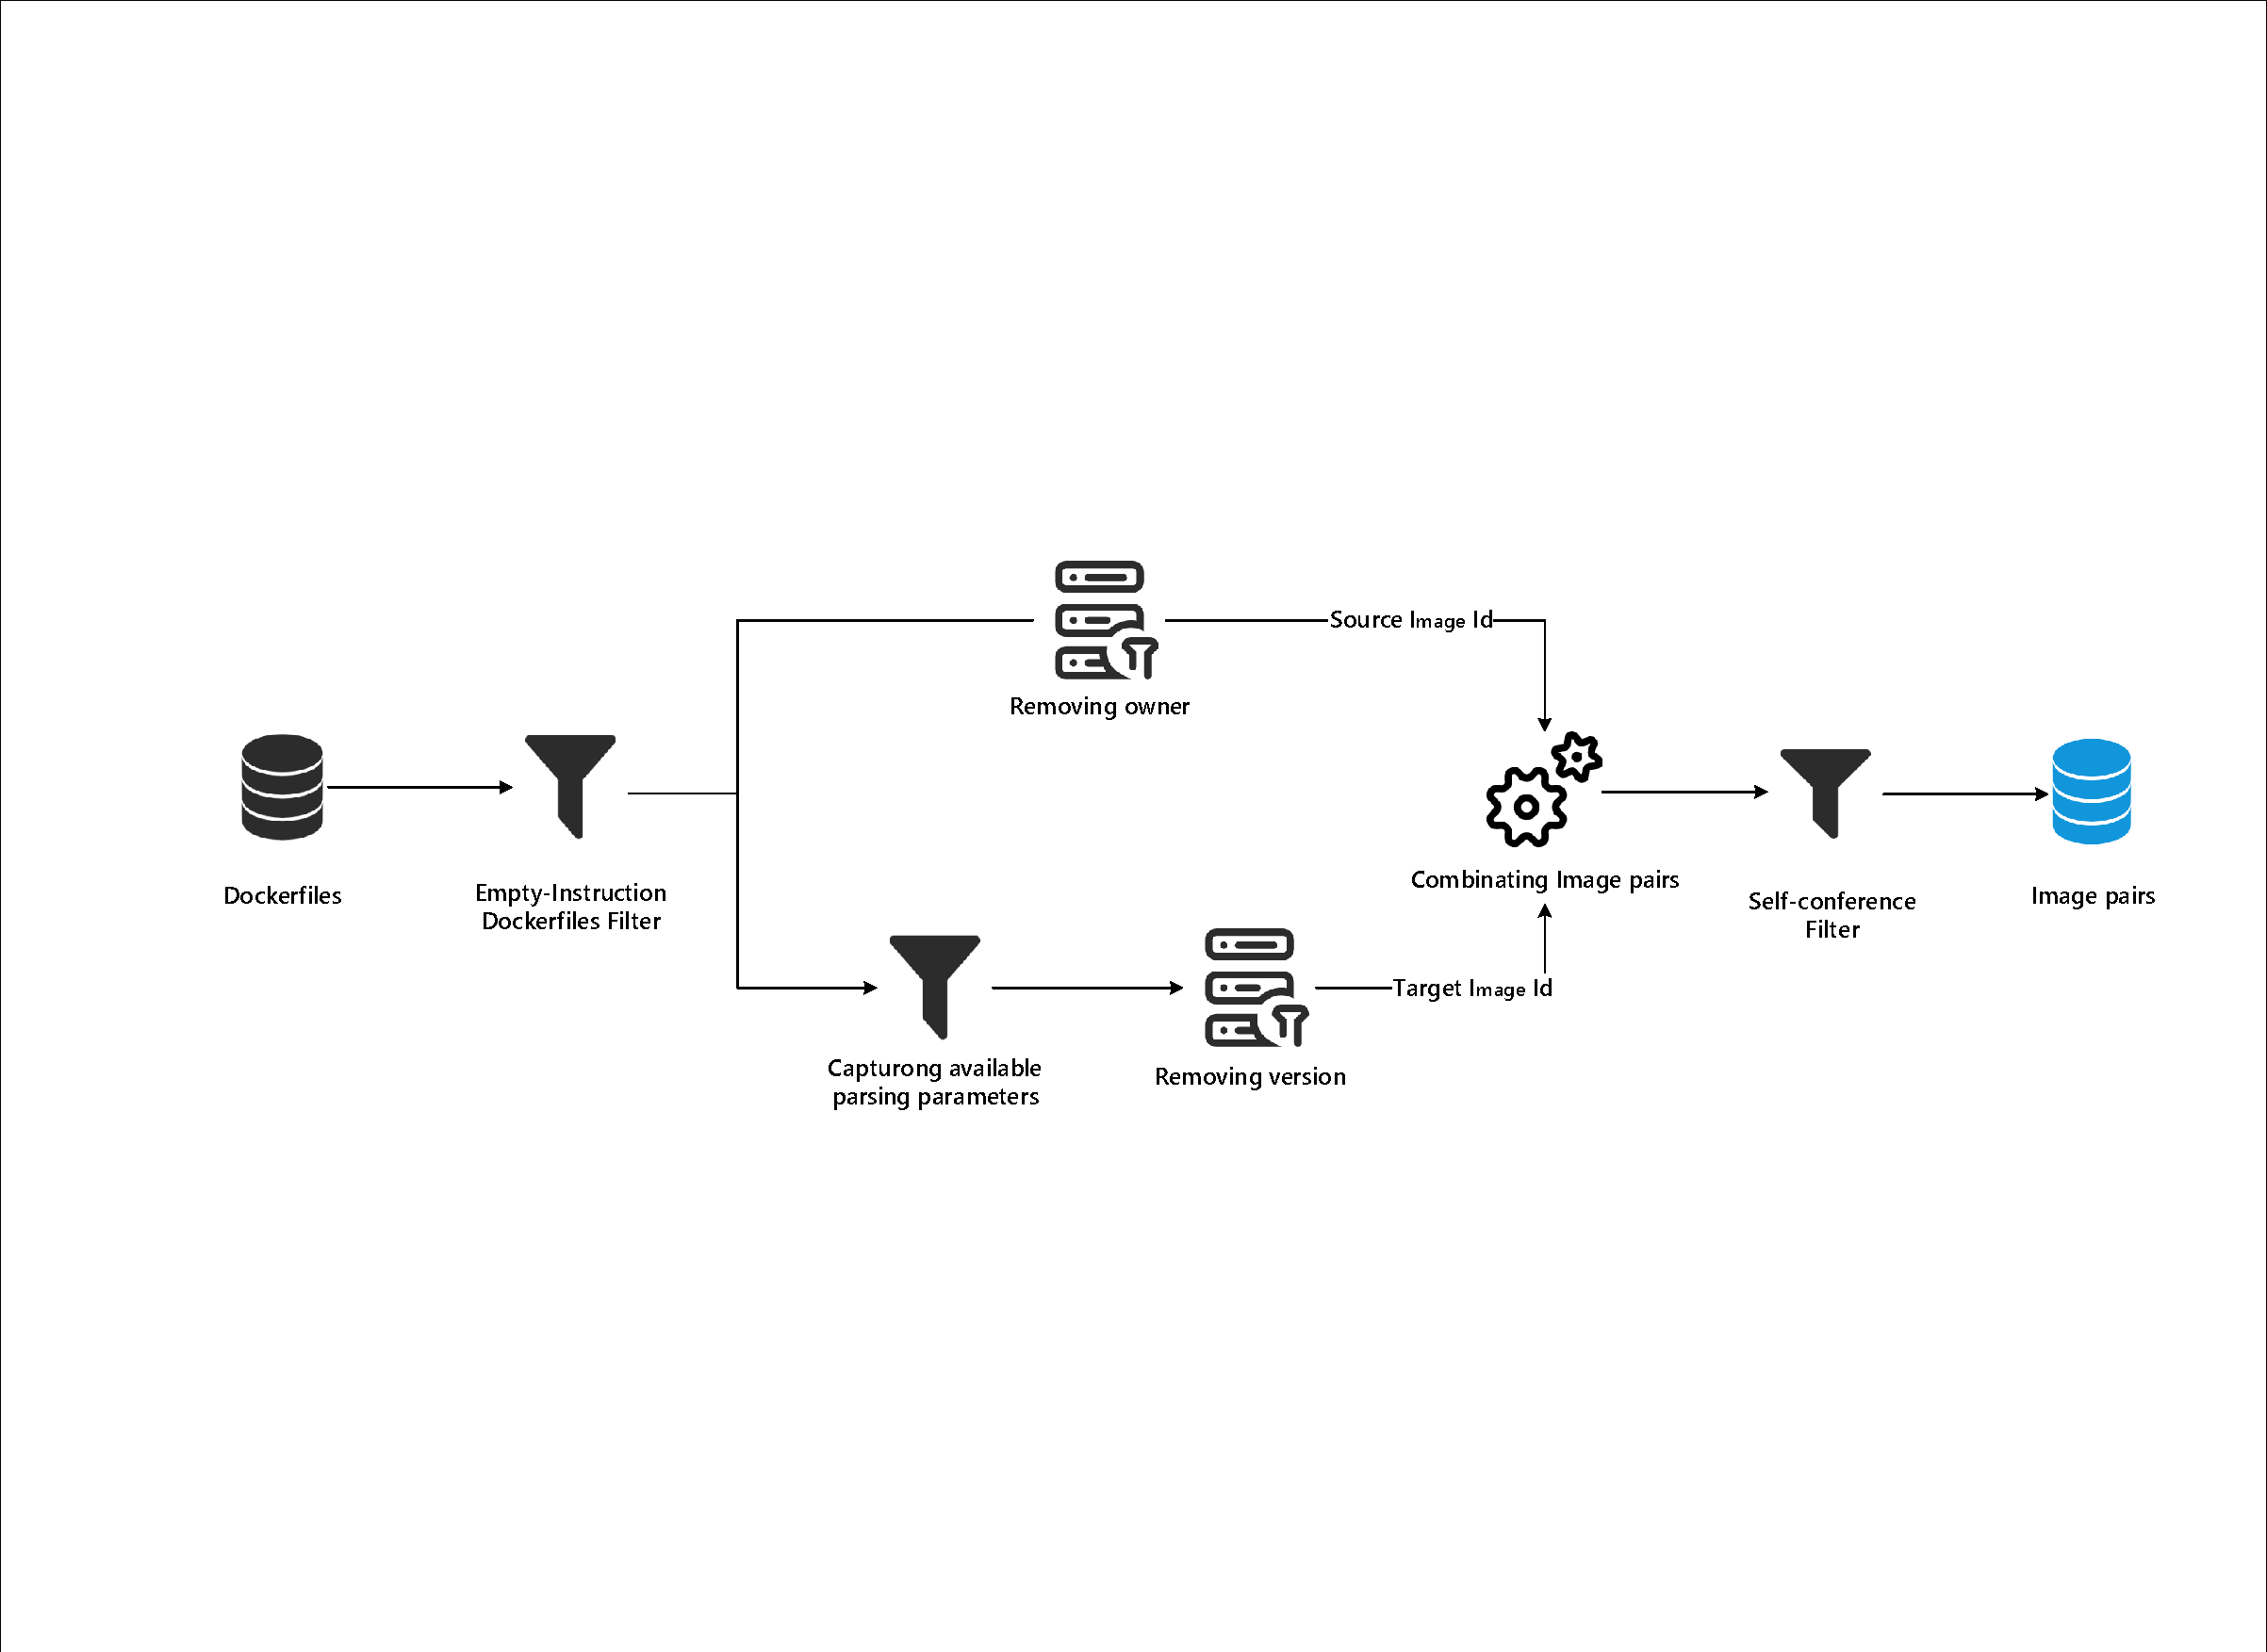
\includegraphics[width=0.6\textwidth,trim=10 270 10 280,clip]{picture//Dataset process.pdf}}
\caption{Procedure of capturing Image Pairs}
\label{fig}
\end{figure}









\subsection{Research Question}
Guided by the purposes of exploring the structre and diversity of docker images network, we proceed along two research thrusts, the first aimed at understanding the structre of overall docker images network that lead to the core images distribution and Quantifies feature, and the second aimed at mining the diversity feature and realitionship of sub-network based on core images.

% We present our study's five key RQs on the structre, diversity and revelence of docker image network, divided into two parts - 

\noindent\textbf{Research Thrust 1. Integral Network Feature Mining.} In this thrust, we character the overall network structre in a progressive way:

\emph{RQ1-1:How is the overall network structre properties presenting?}

\emph{RQ1-2:How is the distribution of docker images divided by degree?}

\emph{RQ1-3:What are those core images?}\\

\noindent\textbf{Research Thrust 2. Sub-Network Linking Relationships Analysis.} 
The core images bringing Attraction and cohesion for Docker Ecosystem prosperity deserve the deeper exploration. Furthermore, we construct and consider within and across dimensions of sub-network:

\emph{RQ2-1:Which are the most tightly connected subnetworks? How do usages affect the structure of subnetworks?}


\emph{RQ2-2:Which are the most tightly connected pair of subnetworks? How do usages affect relationships between subnetworks?}









\section{RT1: Integral Network Feature Mining}

\subsection{RQ1-1:How is the integral network structre properties presenting?}
\noindent\textbf{Motivation. }The initial RQ1-1 aims at understanding the integral network structre. Docker images are not developed isolated that build up realitionships through 
technologial dependence to co-promote the development of docker images. However, even though Docker is widely used in the open-source community, previous research didn't focus on dependency realitionship between docker images. Thus, charactering the network structre properties will help to understand the compactness of the docker images network framework and motivate more work on realitionships of docker images in the future.

\noindent\textbf{Approach. }To address RQ1-1, we primarily use network metric including \emph{node degree} defined as the number of all the nodes point directly to the given node,\emph{diameter} defined as the maxium of the length between any nodes and  \emph{average shortest path} defined as the average of all the length between nodes. Future, we compare the technocial metric of \emph{Image Dependency Network} with other network involving in software projects network and social coding network.

To future present properties of docker images network, we analyzed visualizations of the Dependency Network. We used the Gephi graphing tool to create visualizations.


\noindent\textbf{Results. }The 128,384 link pairs as described in Section  generate 83030 nodes and 98248 edges in the integral docker images network because of the existing of same link pairs.


Figure 1 shows the overall Dependency Network, though for visibility we only display nodes with degree of 10 or greater. From the dimension of interconnection of the integral network, the connections between the core images are apparent.

The diameter calculated is 23 while the average path length is 5.7173. The comparision result of different type of network structre metric showed in TABLE 2 reveal that docker image are actually more interconnected than other networks. The rate of singal-instruction dockerfiles number is 97.85\% of all dockerfiles.

% The reason may be that, on the one hand, ....  A potential explanation is that 
% 2578    220     124384    124384-220-2578=121586    121586-2578=119008 /121586= 97.8%
% 1216    119008-1216=117792/120370 = 97.85% 

\begin{figure}[htbp]
\centerline{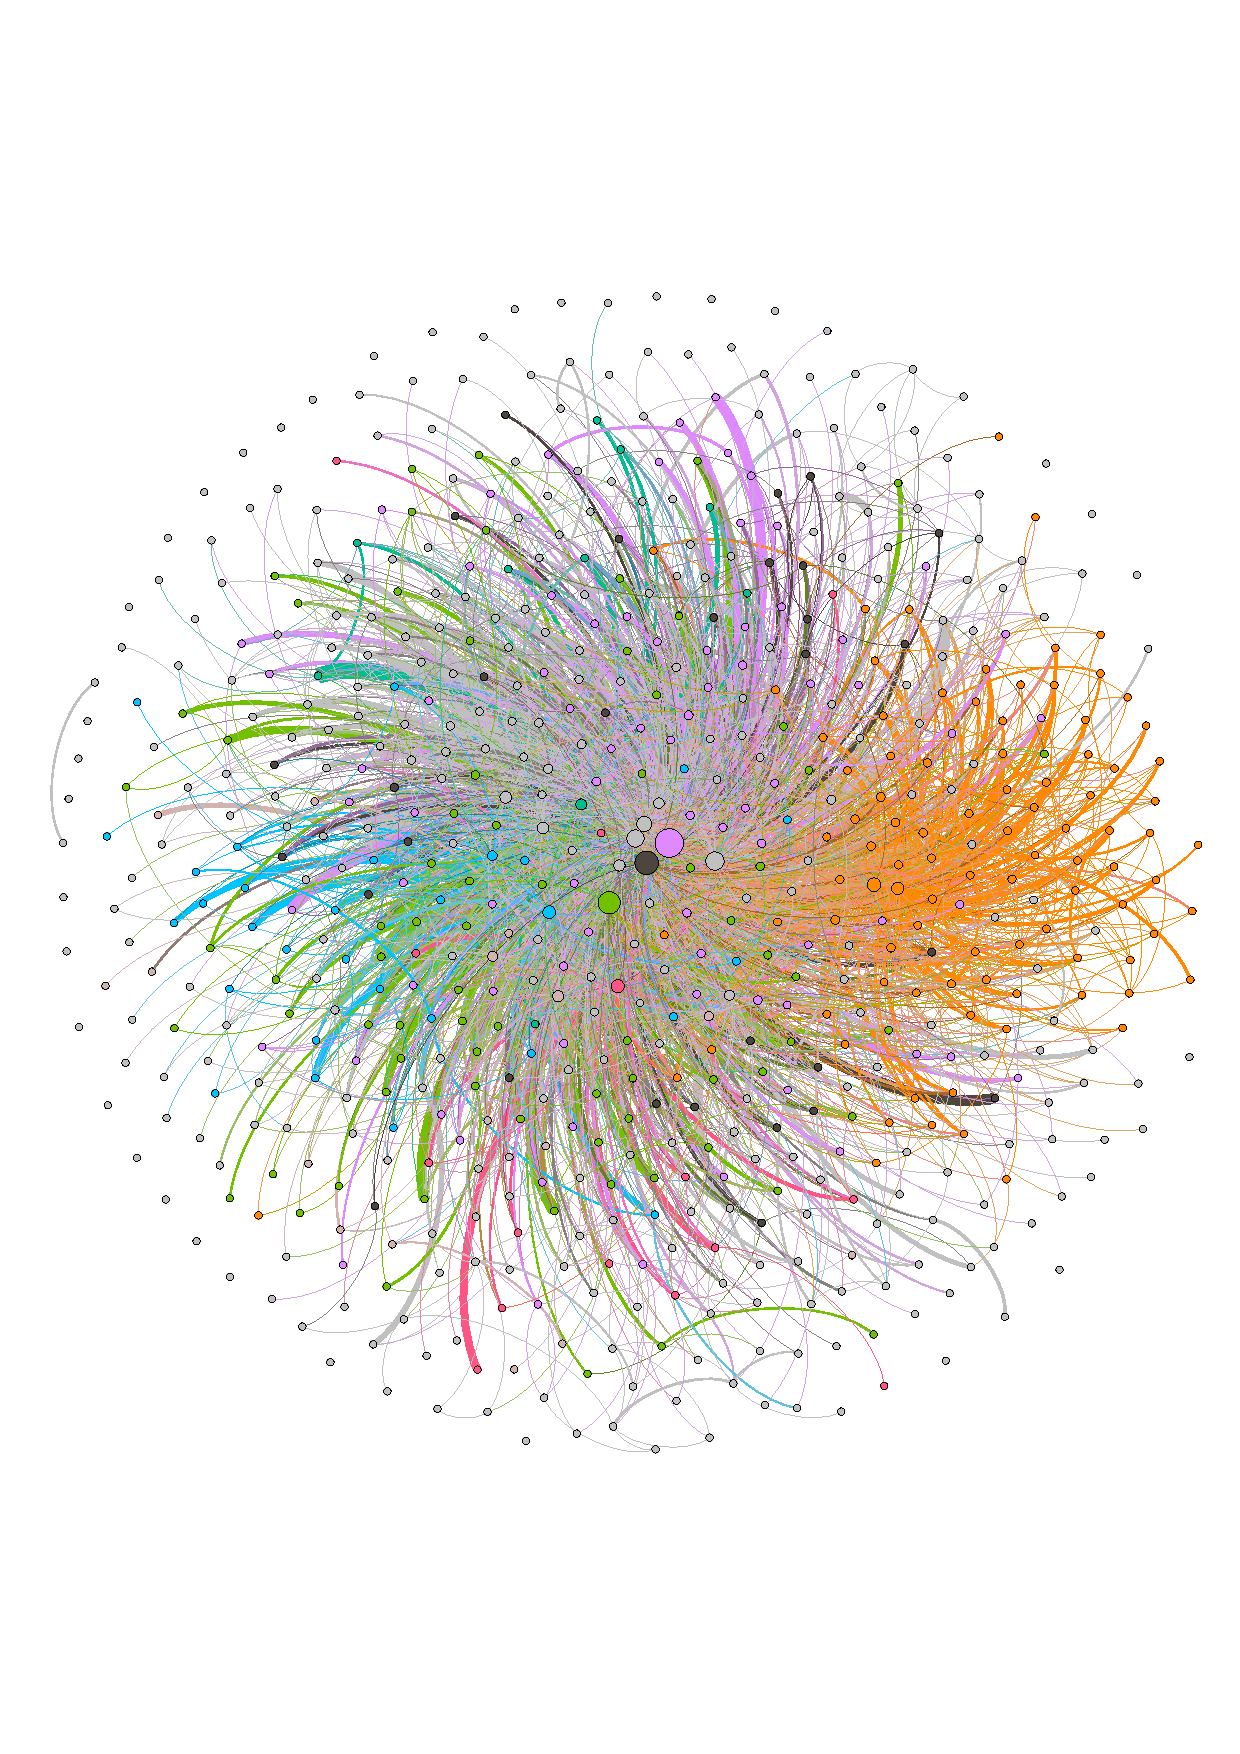
\includegraphics[width=0.5\textwidth,trim=0 130 0 130,clip]{picture//overview_imagenet.pdf}}
\caption{Docker images with dependency realitionships. The size of the node represents the degree of the node, while the thickness of the edge represents the weight of the edge}
\label{fig}
\end{figure}

We compute the diameter valung 21.7 and the average shortest path valuing 5.7 of gaint connected component. Compared with Github projects network and social coding network shown in Table I,docker images network feature larger diameter and average shortest path between nodes.Differ from higher conneted component ration of docker images network,other project networks whose large-scale nodes isolated from giant component shares the average shortest path being 0 with other dis-connected nodes decrease the diameter and average shortest path of the real network.

\begin{mybox}
The interconnection between docker images is relatively loose but reliable. The rate of singal-instruction dockerfiles number is 97.85\% of all dockerfiles.
\end{mybox}


\subsection{RQ1-2:How is the distribution of docker images divided by degree?}
\noindent\textbf{Motivation. }The integral network structre mentioned in RQ1-1 have reveal the apprent interconnection between docker images. Despite the diversity of Docker images, concerns on the regular difference between image nodes well be important, since it helps practitioners find the potential to promote the prevalence of docker images. Thus, this RQ aims to mine the distribution feature of docker images to future explore the distribution difference between docker images.

\noindent\textbf{Approach. }The potential to get insights into the reason for diversity of image ecosystem motivate the exploration of image node distribution. The High degree of node indicate that tight connection between the given node with other nodes but low degree of the given node represent loose connection or nearly isolated with the most nodes, showing that an optimal solution has been found. We futher choose the degree of node as the distribution metic based on high-degree of node represening well-connected of the node. 

The \emph{in degree} of an image is the frequency of other images pointing to the image, the \emph{out degree} of the image is the frequency of the image pointing to other images, and the \emph{degree} of the image is the sum of the \emph{in degree} and the \emph{out degree} of the image.



\noindent\textbf{Results. }The degree distribution across the 83030 images showed as figure 2 follows a typical long tail distribution, 10\% images sharing 90\% degree in intergal docker Image network.         revealing that most dockr images develop relying on several central docker images. This findigs was similar with the conclusion that core project has a powerful appeal to open ecosystem by beida.etc. The reason may be that, on the one hand, 

% talk degree eg..the number of degree=1. 

\begin{figure}[htbp]
\centerline{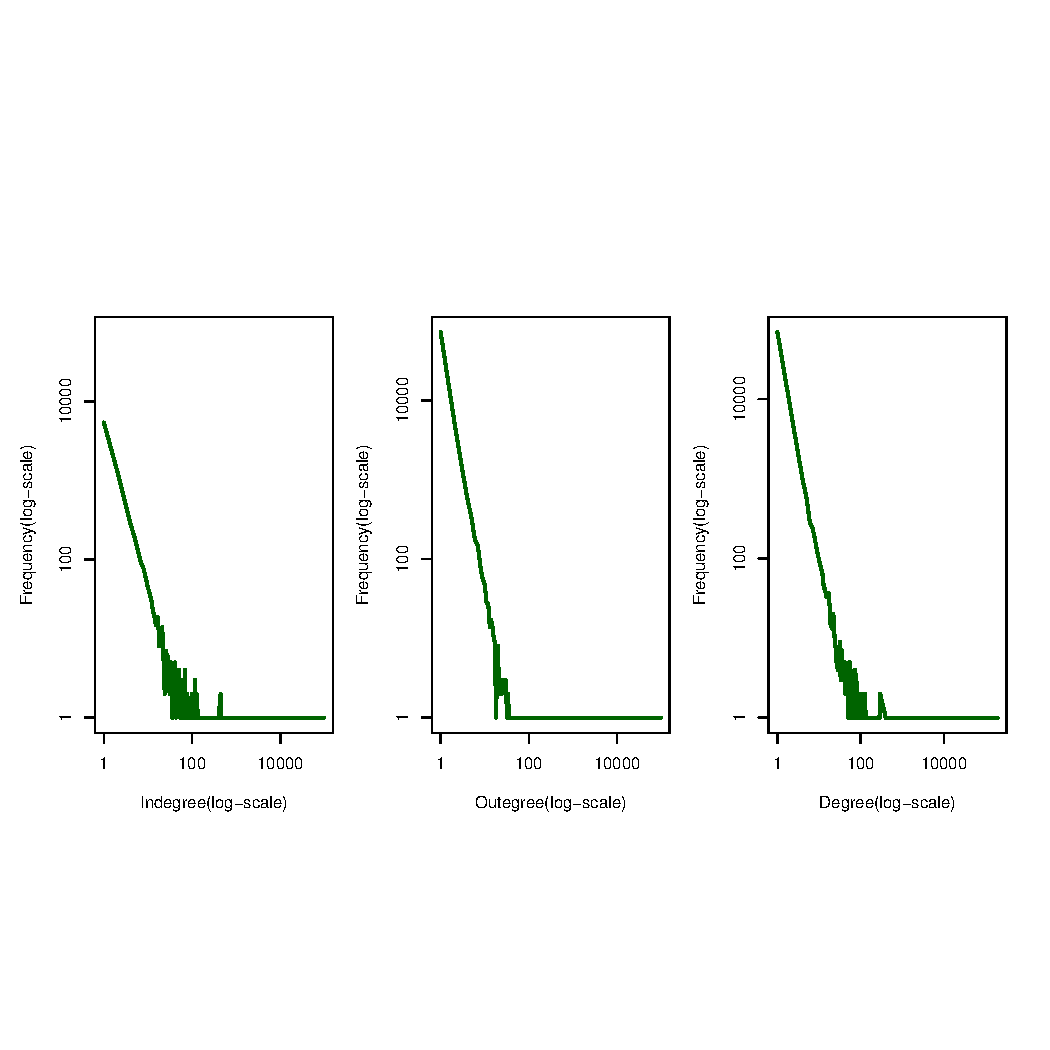
\includegraphics[width=0.5\textwidth,trim=0 90 0 120,clip]{picture//image_distribution_degree.pdf}}
\caption{Docker images distribution by degree}
\label{fig}
\end{figure}

The long-tail images being Cohesiveness and charisma in the network just play an important role in docker images development as the core project promotes the construction of open source ecology.

\begin{mybox}

The long tail distribution 10\% images sharing 90\% degree in docker image network represent the powerful Cohesiveness and charisma of core images to most other images. 
\end{mybox}


\subsection{RQ1-3:What are those core images?}
\noindent\textbf{Motivation. }Despite prevalence of docker ecosystem mainly appealed by core Docker images, however, concerns emerge on the core docker images and why they have strong cohesiveness for Docker ecosystem need further research. This RQ aims at identifying the core images in details. Knowing more information about core images contributes to understand their support for software development. 

\noindent\textbf{Approach. }We say core images are those images with high degree that indicates well-connected images as mentioned above. Further, we ranged and investigate The TOP-100 core images according to the degree of docker images and further compute \emph{in degree}, \emph{out degree} and \emph{degree rate} of the core images. This approach allows to cover significant parts of the overall data, as core images bring prosperity of image ecosystem.  % represent main docker images influence.

\noindent\textbf{Results. }
The TOP-100 influencial docker images, though, occupy the 0.12\% of the number of all images, however, occupy 39.90\% degree of the all degrees. Undoubtedly, this proves the attraction of these 100 core images to other images in the whole ecology. 

Noticely, the indegree of core image is much greater than the outdegree of same images, indicating that each core image occupy the central position with the surrounded other Docker images. The rate of indegree of outdegree is surprsingly reached by 99\% indicating that these core images are always in the central position surrounded by surrounding ambient ordinary images. 


We've only listed the top 20 core images showed as Table1.
Ubuntu images, seen obviously, rank the first docker image stongly over all docker images. Additionally,we find that Operating System always become base images of other images because of debian, alpine, centos included ranking the TOP-10 influencial docker images with high degree.It is also reasonable to hypothesize that, many images choose  Programming language because of their high rate of the influencial images eg..python,ruby. 


Interestingly, these so-called core images are mainly used for support software in the way of software, language or application just look at the 20 core images listed above. 
To further explore the reason for their strong influential in docker images ecosystem






% Table generated by Excel2LaTeX from sheet 'pagerank_degree'
\begin{table}[htbp]
  \centering
  \caption{TOP-20 core images ranked by degree}
    \begin{tabular}{lrrrrr}
\toprule
    Id    & \multicolumn{1}{l}{Indegree} & \multicolumn{1}{l}{Outdegree} & \multicolumn{1}{l}{Degree} & \multicolumn{1}{l}{Degree Rate} \\
\midrule
\rowcolor{mygray}
    ubuntu  & 14,975 & 11    & 14,986 & 7.63\% \\
    alpine  & 8,302 & 5     & 8,307 & 4.23\% \\
\rowcolor{mygray}
    node   & 7,367 & 29    & 7,396 & 3.76\% \\
    debian  & 6,531 & 6     & 6,537 & 3.33\% \\
\rowcolor{mygray}
    python  & 5,883 & 26    & 5,909 & 3.01\% \\
    ruby   & 3,975 & 30    & 4,005 & 2.04\% \\
\rowcolor{mygray}
    centos  & 3,688 & 4     & 3,692 & 1.88\% \\
    golang  & 3293  & 19    & 3312  & 1.69\% \\
\rowcolor{mygray}
    php    & 2,418 & 33    & 2,451 & 1.25\% \\
    nginx  & 1970  & 54    & 2024  & 1.03\% \\
\rowcolor{mygray}
    java   & 1861  & 34    & 1895  & 0.96\% \\
    openjdk  & 1685  & 11    & 1696  & 0.86\% \\
\rowcolor{mygray}
    baseimage  & 1,556 & 9     & 1,565 & 0.80\% \\
    base   & 951   & 34    & 985   & 0.50\% \\
\rowcolor{mygray}
    fedora  & 745   & 2     & 747   & 0.38\% \\
    alpine-node & 720   & 6     & 726   & 0.37\% \\
\rowcolor{mygray}
    scratch  & 681   & 4     & 685   & 0.35\% \\
    maven  & 610   & 12    & 622   & 0.32\% \\
\rowcolor{mygray}
    tomcat  & 445   & 22    & 467   & 0.24\% \\
    buildpack-deps  & 449   & 3     & 452   & 0.23\% \\
\bottomrule
    \end{tabular}%
  \label{tab:addlabel}%
\end{table}%


\begin{mybox}
The TOP-100 influencial docker images, though, occupy the 0.12\% of the number of all images, however, occupy 39.90\% degree of the all degrees. The rate of indegree of outdegree is surprsingly reached by 99\% indicating that these core images are always in the central position surrounded by surrounding ambient ordinary images. 
\end{mybox}





































\section{RT2: Diversity and Relevance between sub-networks:core image}
% Differences and connections

The characteristics of the overall network have been answered through RT1, RT2 will further conduct empirical analysis on the structure, diversity and relevance of network based on core images.  To investigate/summarize the character of diversity and relevance of subnetworks of coreimage, we investigate/analyse differences and connections between subnetworks using network and classify metricc.


%Our empirical study in RT1 reveals that the role of singal core image in software development and interestingly discover the star linking pattern due to the high indegree of these core images.





%in order to better understand core images from linking angle, exploring the image itself is not enough. Based on the high indegree of core images, we construct sub-network centraled with core images aiming at investigating differences and connections between sub-network of coreimages.

%We have known the importance of the core images and further conduct research on their usage for software development. A single image is by no means the end, however, we need conduct deep study to realte images that have dependency realitionships with core images to get insights into the core images realted.  To get a better understanding of core images from the perspective of the network, we construct the networks centered on singal core image. 



% much more tightly connected 


%\subsection{Sub-network:coreimages Statistics}Sub-network defined by directing directly or directing indirectly in the way of multiple FROM instruction spread to the influencial images can be symbolized as a set of vector. Under this definition, we can classify the interconnection of sub-network into three categories:(1)none internection:images in this sub-network all direct to this offical images which didn't rely on any docker image. (2)direct dependency connection:the core influencial image also direct to other images. (3)indirect dependency connection:the influencial centraled by other images didn't direct other images, however, being directed by other image directing other image in one dockerfile.     




\subsection{RQ2-1:  Which are the most tightly connected subnetworks?}\label{AA}


\noindent\textbf{Motivation. }Supporing research on the follow-up RQs motivates this RQ to construct subnetworks of core images and explore deeply usage of subnetworks for supporting software development. Idendifying these subnetworks included subnetworks structre and subnetworks type is conductive to understand the way and to what extent they promote the development of software and docker ecosystem. 


%the way of        To future explore the propertioes and usage of core images for supporting software development, we construct subnetwork surrounded with core images and classify type of subnetworks.  This RQ aimes at idendifing TOP-20 compensess subnetworks and exploring the way of all subnetworks of core imaegs supporting for software development.   

\noindent\textbf{Approach. }To address this RQ, our approach includes the following detailed steps.

\noindent\textbf{Step1:Construct \emph{Subnetwork:core image }}Based on the attraction to the whole ecosystems of core images, we selected TOP-100 core images obtained by RQ1-3 from all images, and future construct 100 subnetworks surrounded with them. 
To realted images that have dependency realitionships with core images and consider the star pattern of core images, we define \emph{Subnetwork:core image} as a directed graph \emph{SN$_d$} = $\left \langle V,E \right \rangle$ indicating the network structre of subnetwork. The set of vertices, denoted by V, is the number of all docker images directing core image and the core image itself. The set of edges, denoted by E, is the directed links between images in this subnetwork. is a set of node pairs \emph{E(V)} = $\left\{ 	\left( Ii, Ij \right)|Ii,Ij \in E. \right\}$. If the project represented by node xicross-referenced the
project represented by node yj, there is a directed edge from Ii to Ij. The weight of each edge is the count of cross-references for the pair of projects. 

% yu dataset corresponding 


%labeld by link times. eg.. ubuntu directed to php in different dockerfile for 4 times, the label of this edge is 4.



%fistly construct subnetworks surrounded with core images. We construct the subnetwork revolving around core image based on the star pattern presented by linking between core images and around images. \emph{in degree} 




\noindent\textbf{Step2:Classify For Subnetwork Type}
Consider the core image centraled in subnetwork, we say the type of subnetwork being the type of core image in this subnetwork.
To further explore the reason for strong influential of subnetworks in docker images ecosystem, we firstly manually categorize the docker core images into 5 types including Operating System marked as OS, Program Language marked as LR, Tools/Services marked as T/S, Application Instructre/Framework marked as AI/F. according to their practical usage based on the images tag by Docker Hub and study of Jürgen Cito etc.
Specificly, "OS" are images that manages computer hardware, software resources, and provides common services for computer programs."Language runtime", in addition, contain a runtime needed to execute applications written in a specific programming language. "Tools/Services" are images that , for example, a database, DevOps Tool or a Web server. "Application I/F" are base application Infrastructure or Frameworks that bring Fourth Industrial Revolution to Infrastructure. Specially, "Other" denotes images that do no fit cleanly into any of the above categories, for example scratch, an empty image, or busybox, a collection of UNIX utilities or base, a variable is impossible to explore its exact type. % \%70 are offical images, the other are some private images.

 %step 1 step 2.
Then two experienced developers were invited to classify the 100 images separatly at the same time, and only three classifies are different that this classification can be considered valid.

 

 
\noindent\textbf{Step3:Select Subnetwork Metics} To character structre of subnetworks, we use metrics invoving Nodenumber, EdgeNumber, Edges to evaluate scale of subnetworks and use Edges/Nodenumber metric to evaluate network compactness. Noticely, we gave up using it diameter, pathlength frequently-used network metics to evaluate compactness of subnetworks due to inapplicability to our network structre after a series of experiments. The potential reason is that our subnetworks always present as star pattern. The compuate of Diamter is only consider on connecting points while links between images directing core images in star pattern subnetworks result diameter and avg.length bigger that contradicted with the fact of compactnesser subnetwork structre. However, Edges/Nodenumber identifying the rate of linking frequency with images number seems both direct and appropriate metic in charactering star pattern subnetworks.   


\begin{figure}[htbp]
\centerline{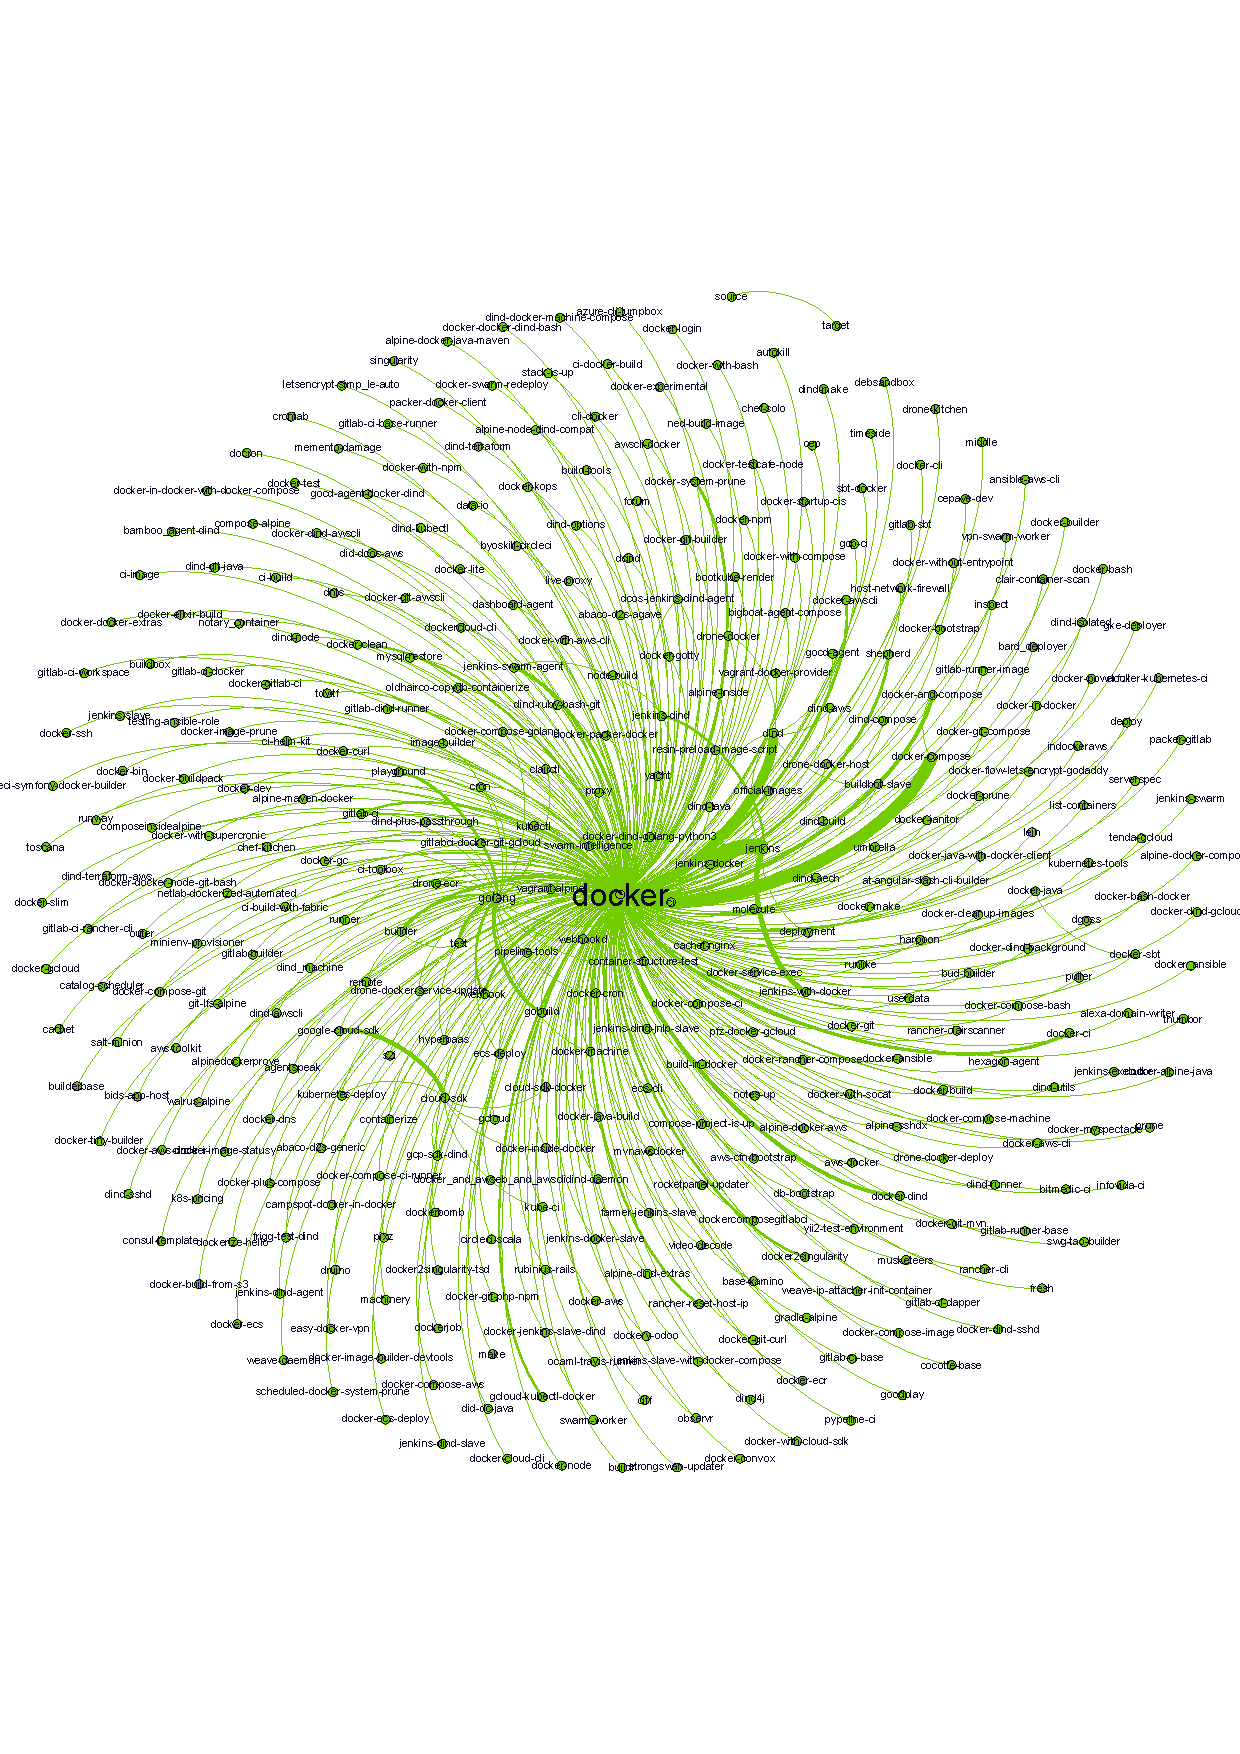
\includegraphics[width=0.4\textwidth,trim=0 130 0 130,clip]{picture//image_network_docker.pdf}}
\caption{SubNetwork:docker}
\label{fig}
\end{figure}

% Table generated by Excel2LaTeX from sheet 'Sheet2'
\begin{table}[htbp]
  \centering
	\small
  \caption{TOP-20 Clostest Subnetworks}
    \begin{tabular}{llrrrr}
\toprule
    Subnetwork\_id & Type  & \multicolumn{1}{l}{\#Nodes} & \multicolumn{1}{l}{\#Edges} & \multicolumn{1}{l}{\#Links} & \multicolumn{1}{l}{\#Links/\#Nodes} \\
\midrule
    buildpack-deps & Other & 450   & 852   & 2191  & 4.869  \\
    baseimage & Other & 1557  & 2642  & 5950  & 3.821  \\
    base  & Other & 952   & 1720  & 3295  & 3.461  \\
    apache & T/S   & 71    & 93    & 245   & 3.451  \\
    centos7 & OS    & 68    & 93    & 230   & 3.382  \\
    scratch & Other & 681   & 1102  & 2214  & 3.251  \\
    alpine-glibc & OS    & 165   & 240   & 508   & 3.079  \\
    alpine-java & LR    & 194   & 275   & 586   & 3.021  \\
    opensuse & OS    & 100   & 144   & 299   & 2.990  \\
    base-alpine & OS    & 70    & 88    & 198   & 2.829  \\
    ubuntu & OS    & 14976  & 22535  & 38577  & 2.576  \\
    openjdk & LR    & 1686  & 2437  & 4328  & 2.567  \\
    composer & T/S   & 125   & 183   & 315   & 2.520  \\
    alpine & OS    & 8303  & 12222  & 20395  & 2.456  \\
    cuda  & AI/F  & 278   & 346   & 668   & 2.403  \\
    debian & OS    & 6532  & 9571  & 15671  & 2.399  \\
    openresty & T/S   & 67    & 72    & 160   & 2.388  \\
    centos & OS    & 3689  & 5273  & 8630  & 2.339  \\
    alpine-oraclejdk8 & LR    & 126   & 150   & 261   & 2.071  \\
    fedora & OS    & 746   & 962   & 1533  & 2.055  \\
\bottomrule
    \end{tabular}%
  \label{tab:addlabel}%
\end{table}%



%% Table generated by Excel2LaTeX from sheet 'Sheet1'
%\begin{table}[htbp]
%  \centering
%  \caption{Core image type count in TOP-100}
%    \begin{tabular}{lrrrrr}
%\toprule
%    Type & \multicolumn{1}{l}{Tools/Services} & \multicolumn{1}{l}{OS} & \multicolumn{1}{l}{LR} & \multicolumn{1}{l}{Application I/F} & \multicolumn{1}{l}{Other} \\
%\midrule
%    count & 42    & 21    & 18    & 11    & 8 \\
%\bottomrule
%    \end{tabular}%
%  \label{tab:addlabel}%
%\end{table}%





%\begin{figure}[htbp]
%\centering
%\begin{minipage}[t]{0.2\textwidth}
%\centering
%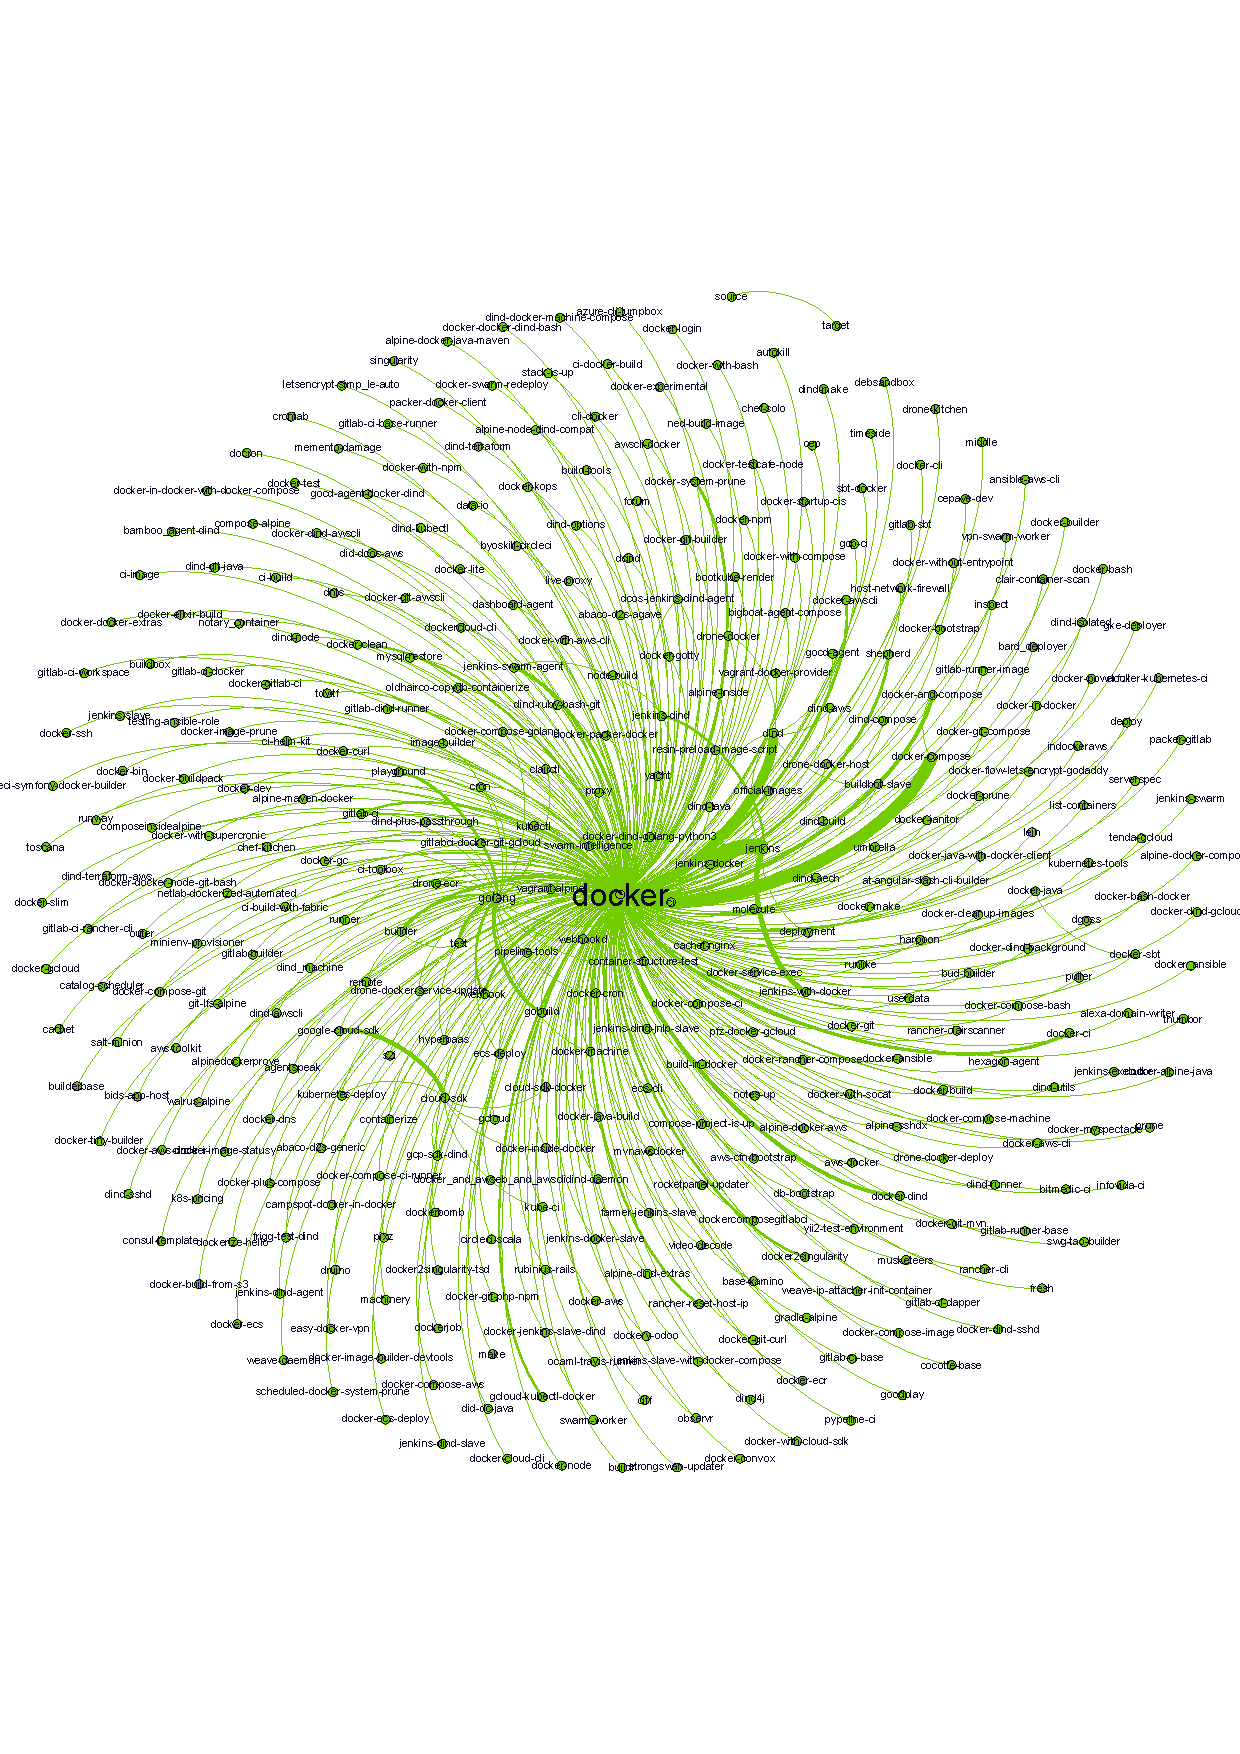
\includegraphics[width=1\textwidth,trim=0 130 0 130,clip]{picture//image_network_docker.pdf}
%\caption{W}
%\end{minipage}
%\begin{minipage}[t]{0.2\textwidth}
%\centering
%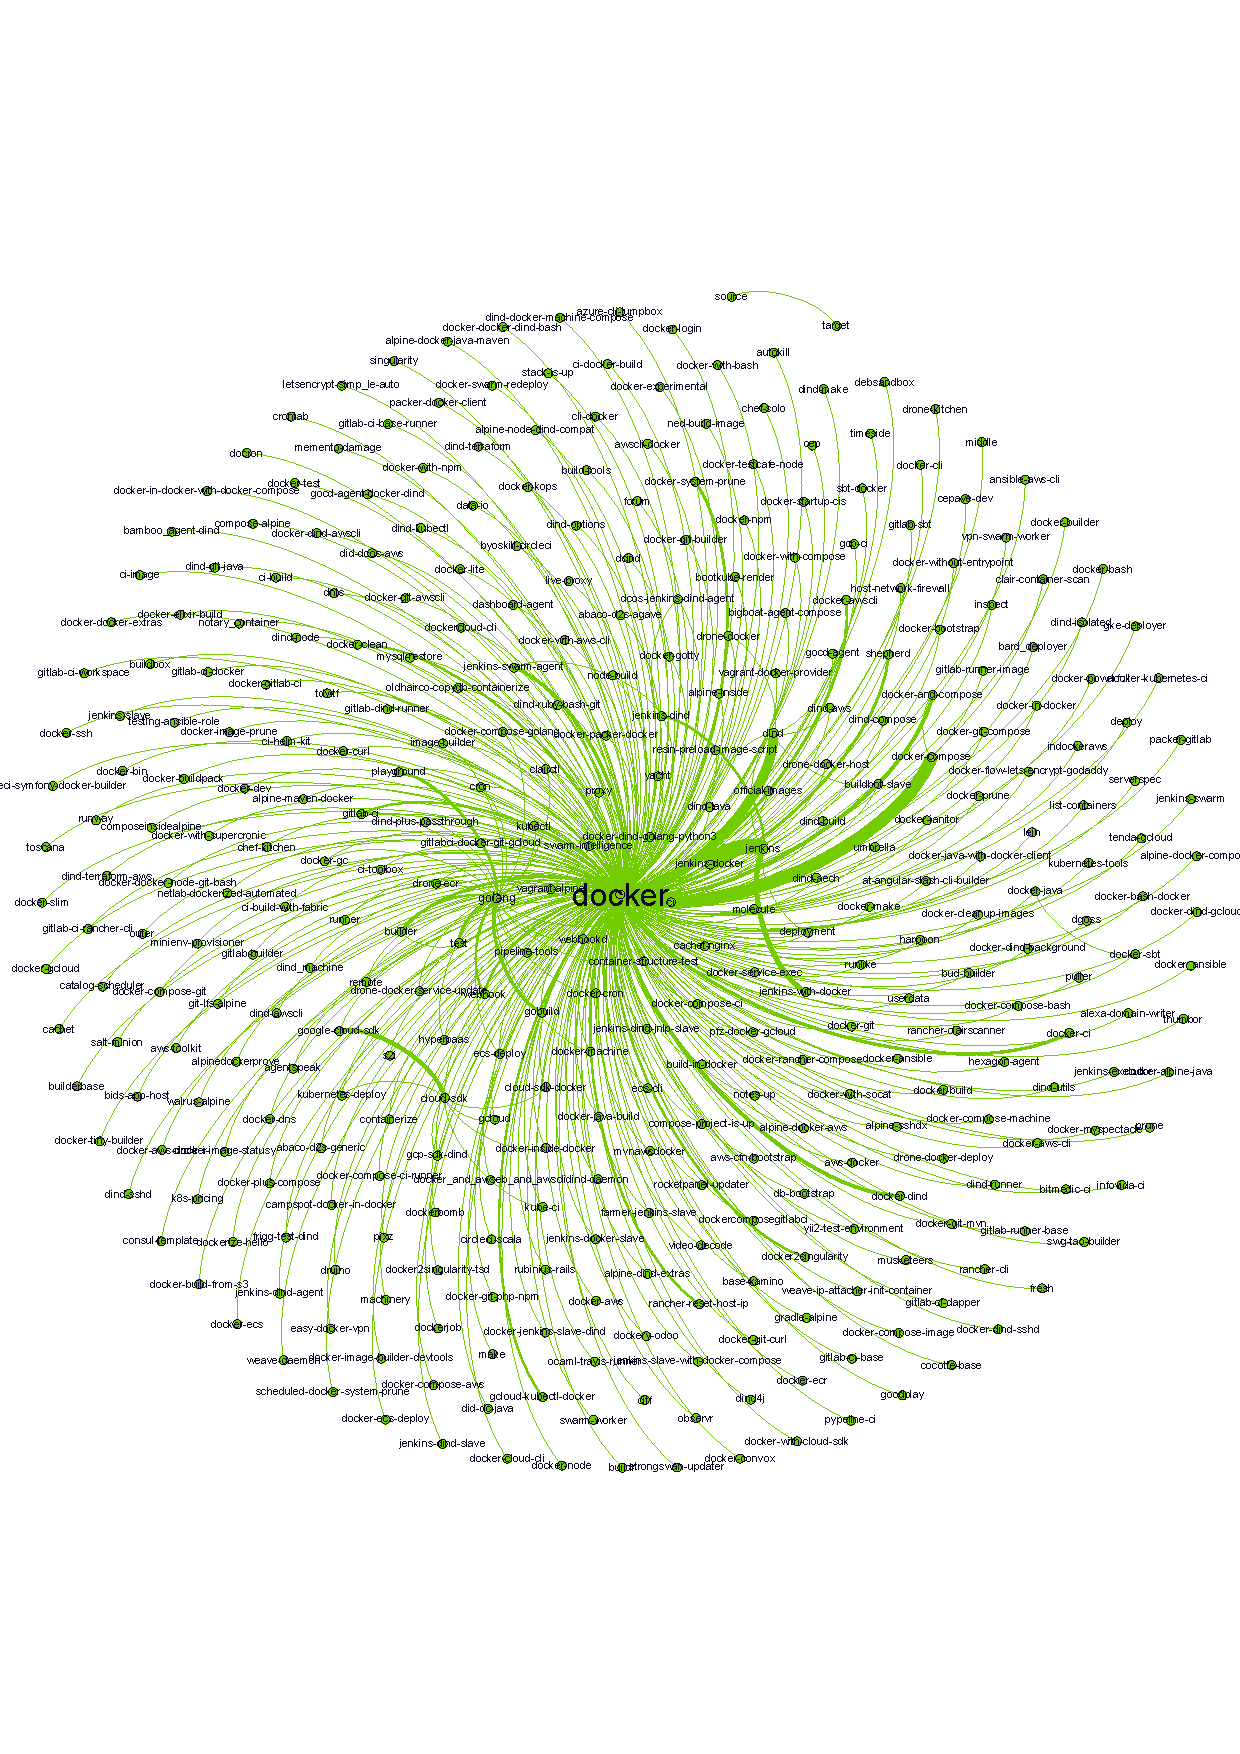
\includegraphics[width=1\textwidth,trim=0 130 0 130,clip]{picture//image_network_docker.pdf}
%\caption{C}
%\end{minipage}
%\end{figure}





\noindent\textbf{Results. }
Figure4 gives an example of subnetwork:docker we constructed, core image-docker, occupying the center of the subnet, part of images, also connected with each other. 
Detailed metic information,in addition, can be seen in Table 2 ranked by Links/Nodes. Subnetwork:buildpack-deps, As the image build instruction set, has the most interconnected network structre, but scale is average. Subnetwork:ubuntu, the most biggest in all subnetworks, has the high internal interconnection.

Interestingly,  we find these \emph{subnetwork:core images} are mainly used for support software or images development. Detiled, of the TOP-100 \emph{subnetwork:core images}, there are 42 Tools/Services, 21 OS, 18 Language runtime and 11 Application I/F.  



\begin{mybox}
These \emph{subnetwork:core images} are mainly used for support software or images development. Detiled, of the TOP-100 \emph{subnetwork:core images}, there are 42 Tools/Services, 21 OS, 18 Language runtime and 11 Application I/F.
\end{mybox}










\subsection{RQ2-2:  How do usages affect the structure difference of subnetworks?}\label{AA}
\noindent\textbf{Motivation. } RQ2-1 has identified several detailed subnetworks and gave interpretable metics to evaluate properties of subnetworks. To future understand properties presented by different subnetworks,  carrying out specific empirical research is essential. Thus, this RQ aims at investigating how and to what extend subnetworks perform diversity in scale, interconnectedness of subnetworks differed in usage type to give insights into the properties of subnetworks. 


%Investigating the most tightly subnetworks in details is conducive to further obtain common feature and understand the reason for being tight subnetworks. 

% In addition, Sub-networks constructed by different type influencial images may undertake different functional aids in promoting docker images universal and mantainced. Guide by the rule, we divide the influencial images into several types including Operating System, Program language, Application service, Application framework etc as the TABLE 2 clearly shows. 


%However, differences scale and compactness of subnetworks may present a varirty of features, therefore it is important to investigate how and to what extend subnetworks performance diversity.

\noindent\textbf{Approach. }
To assess the change in subnetwork type diversity, we aggregate our dataset per type of usage for software development to obtain the scale and interconnectedness metic across subnetworks type. For each subneytwork type, we compute the the nodesnumber, edgesnumber and linksnumber of each subnetwork. 
To elaborate the reliability of the results, we apply Kruskal-Wallis test to assess and also apply Wilcoxon test and Cliff’s delta library(effsize) to assess difference between two samples. 

% picture for star pattern subnetwork




\begin{figure*}[htbp]
\centerline{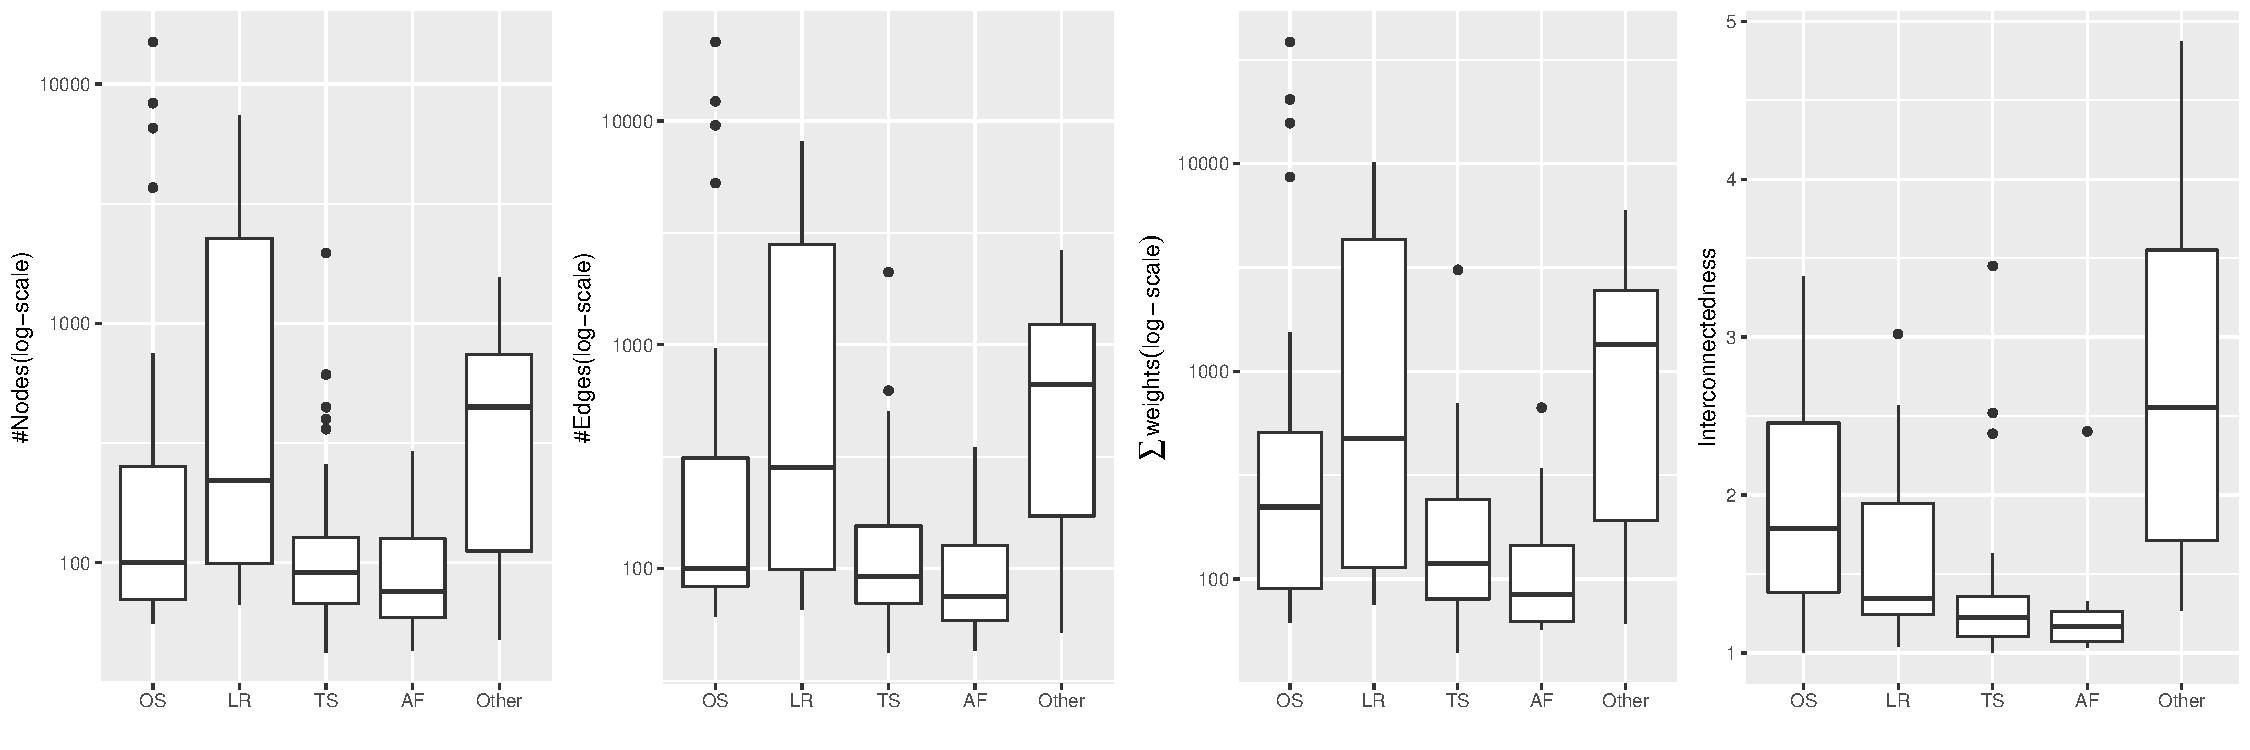
\includegraphics[width=1\textwidth]{picture//sub_coreimages_netstructre.pdf}}
\caption{Subimages Net Structre In Group2}
\label{fig}
\end{figure*}









\noindent\textbf{Results. }The TOP-20 image, ranked by avg.edge can be showed attached with realted metic information in TABLE 2. Apache, as a famous web server, has the clostest realitionships within its subnetwork with the Avg.edge being 2.634. 


Further, we compared diameter and average shortest length of the divided image groups. Figure 3 shows the comparison boxplots. We find that different typse of influencial images network may have different network structre. E.g.,Operating system sub-network may have larger diameter and average shortest length. This may result from Operating system's larger sub-network scale. Because of the build-form of the sub-network always character as the star pattern(large amount of docker images always central with one or minority docker images)  


As fig3 shows, Language Runtime has largest nodenumber and edgenumber while Application I/F has the smallest nodenumber and edgenumber among all images type that defend the scale of the various types of all images. Interestingly, OS ranked the second among the four images types but with several abnormity
images including ubuntu, alipine etc. The reason may be that these several abnormity images are extremely popular compared with another OS images. The real biggest scale are these several operating system based on linux system. Actually, the scale of these sub network of core images reflect the usage 
frequency of core images by other images. 

Noticely, the rightest sub picture in fig3 reflect the degree of association within sub-networks. OS has the strongest compactness, followded by Language Runtime. Meanwhile, the Application I/F has the loostest structre among the four types.

The real meaning of avf.length is the linking frequency between images within the sub-network of core images. Different dockerfile may reference images with the same main body that reflect the compactness of sub-network. 


% here need a sample of singal docker images to show off 


\begin{mybox}
Language Runtime has largest nodenumber and edgenumber while Application I/F has the smallest nodenumber and edgenumber among all images. Interestingly, OS ranked the second among the four images types but with several abnormity images including ubuntu, alipine etc. OS, in addition, has the strongest compactness, followded by Language Runtime.
\end{mybox}







%\subsection{RQ2-2:How is the link pattern between sub-network of images?}
%The sub-network of the docker images, interestingly, interactive with other sub-network not singlely. We divided the interactive mode into three patterns shownd as figure4. 


%\noindent\textbf{none internection:} witout exist 

%\noindent\textbf{direct dependency connection} rank

%\noindent\textbf{indirect dependency connection}

%On average, 70\% interconnected mode of sub-network were none internetection, 20\% mode were direct dependency connection and 10\% mode were indirect dependency connection. It is worth mentioning that the inter cause of the indirect dependency connection is the two or more FROM instruction in the same dockerfile.




%\begin{mybox}
%4!!!!!!!!!!!!! modes   not 3!!!!!!
%none connection 3    only indirect 3    only direct 32    both connection 62
%3+3+32+62 =100
%\end{mybox}













\subsection{RQ2-3:Which are the most tightly connected pair of subnetworks? How do usages affect relationships between subnetworks?}
Base on the above analyse, it is the several From instructions that resulting the interactive realitionships between docker images. To further explore the stronger realitionship between sub-networks and the several FROM instructions distribution and reasons between docker images, we list the TOP-20 strongest realtionships between docker images as TABLE2 shows.


\noindent\textbf{Motivation. }
Diversity of subnetworks, foucsing on differences in size and compactness within subnetworks has been  investigated in depth in RQ2-1. Since core images are proved not to be isolated, therefore we also have reason to believe the revelence relationships between subnetworks.  However, deep insights into the tightly connected subnetworks pairs and the effect of use on the revelence relationshps need the further research. By answering these questions, we can perceive the overview of realitionships between different type of subnetworks. The stronger realitionships pairs captured may be a singal of coorporate realitinshp for software development. We can use it to capture the realitionships feature for images recommendation according to their similar feature or coorporate feature.



%Core images may directed to other images belonging to other sub-network, One image, interestingly, may direct to different images belonging to different sub-networks that reflect sub-networks are not isolated. Further, deep insights into the more stronger realitionships is           
%necessary. In other words, 

\noindent\textbf{Approach. }
The \emph{linking strength} emerges from linking frequency between the intersection of two subnetworks with the two core images, defined as ...
Intuitively, the cross spots belonging to two subnetworks meanwhile represent linking realitionships between subnetworks. Further, we defined the \emph{linking strength} between subnetworks as the the edges times between crossspots and core images multipy frequency labels, symbolized as \emph{linking strength} = \emph{edge} * \emph{timeslabel}. 

In order to explore the influence of core image type on subnetworks, we study in depth the rules and features of different types of subnetworks linking relationships. The subnetwork pairs, can be classified by type of core image according to the usage for software development mentioned above, eg..OS-OS for image pair (alpine,ubuntu).  Noticely, we say type of subnetworks Pairs containing subnetwork classified as other as Other-.




\noindent\textbf{Results. }Interconnection of 100 subnetworks centraled with TOP-100 core images result 4950 Subnetwork Pairs.  Showed as Table 4, TOP-20 most tightly linked subnetworks pairs can be obviously observed attached with \emph{linking strength} and \emph{Type-Pairs} results. 
We also Statisticed the most noteworhty TOP-100 subnetwork pairs, the count of subnetwork pairs type among them are given as TABLE 5. OS-LR OS-OS are most tightly connected subnetwork pairs, followed by LR-LR and OS-TS. 


\begin{figure}[htbp]
\centerline{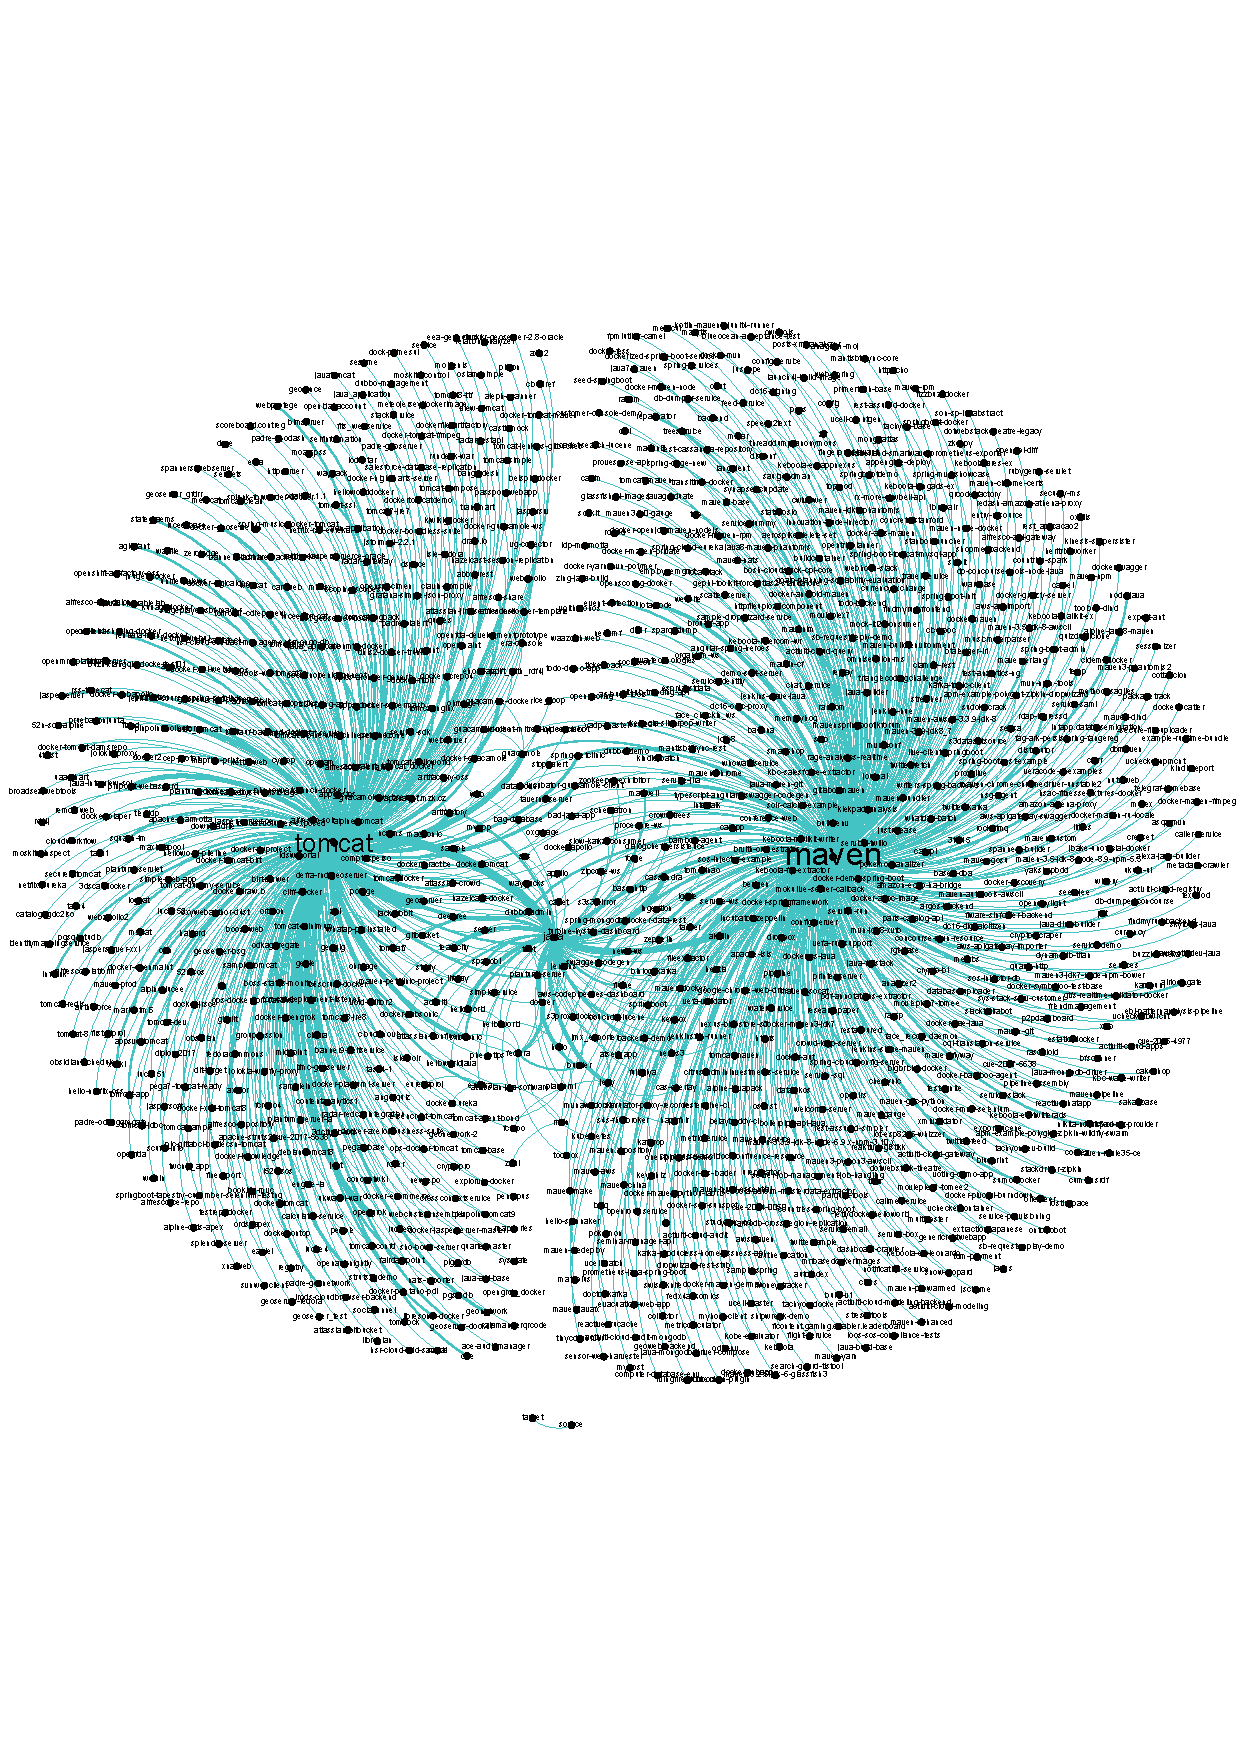
\includegraphics[width=0.4\textwidth,trim=0 130 0 130,clip]{picture//image_network_pairs_maven_tomcat3.pdf}}
\caption{SubNetwork:maven--SubNetwork:tomcat}
\label{fig}
\end{figure}




% Table generated by Excel2LaTeX from sheet 'coreimages_network_crossspots'
\begin{table}[htbp]
  \centering
  \caption{TOP-20 linking strength subnetworks}
    \begin{tabular}{lllr}
	\toprule
    coreimage1 & coreimage2 & Type-Pairs & \multicolumn{1}{l}{linking strength} \\
	\midrule
    ubuntu & alpine & OS-OS & 7,487 \\
    ubuntu & debian & OS-OS & 7,391 \\
    alpine & debian & OS-OS & 5,665 \\
    ubuntu & centos & OS-OS & 4,194 \\
    golang & alpine & OS-LR & 2,833 \\
    ubuntu & baseimage & Other- & 2,772 \\
    ubuntu & base  & Other- & 2,550 \\
    centos & alpine & OS-OS & 2,523 \\
    node  & ubuntu & OS-LR & 2,329 \\
    centos & debian & OS-OS & 2,329 \\
    python & ubuntu & OS-LR & 2,303 \\
    alpine & base  & Other- & 2,095 \\
    ubuntu & java  & OS-LR & 1,925 \\
    alpine & baseimage & Other- & 1,905 \\
    php   & ubuntu & OS-LR & 1,881 \\
    baseimage & debian & Other- & 1,791 \\
    python & alpine & OS-LR & 1,775 \\
    base  & debian & Other- & 1,751 \\
    java  & openjdk & LR-LR & 1,688 \\
    ubuntu & openjdk & OS-LR & 1,558 \\
	\bottomrule
    \end{tabular}%
  \label{tab:addlabel}%
\end{table}%




\begin{table}[htbp]
  \centering
	\small
  \caption{Subnetworks type count in TOP-100}
    \begin{tabular}{lrrrrrrr}
\toprule
    Type & \multicolumn{1}{l}{OS-OS} & \multicolumn{1}{l}{OS-LR} & \multicolumn{1}{l}{LR-LR} & \multicolumn{1}{l}{OS-TS} & \multicolumn{1}{l}{LR-TS} & \multicolumn{1}{l}{OS-AI/F} & \multicolumn{1}{l}{Other-} \\
\midrule
    count & 28    & 30   & 7    & 7  & 2  & 1 & 25 \\
\bottomrule
    \end{tabular}%
  \label{tab:addlabel}%
\end{table}%




\begin{figure}[htbp]
\centerline{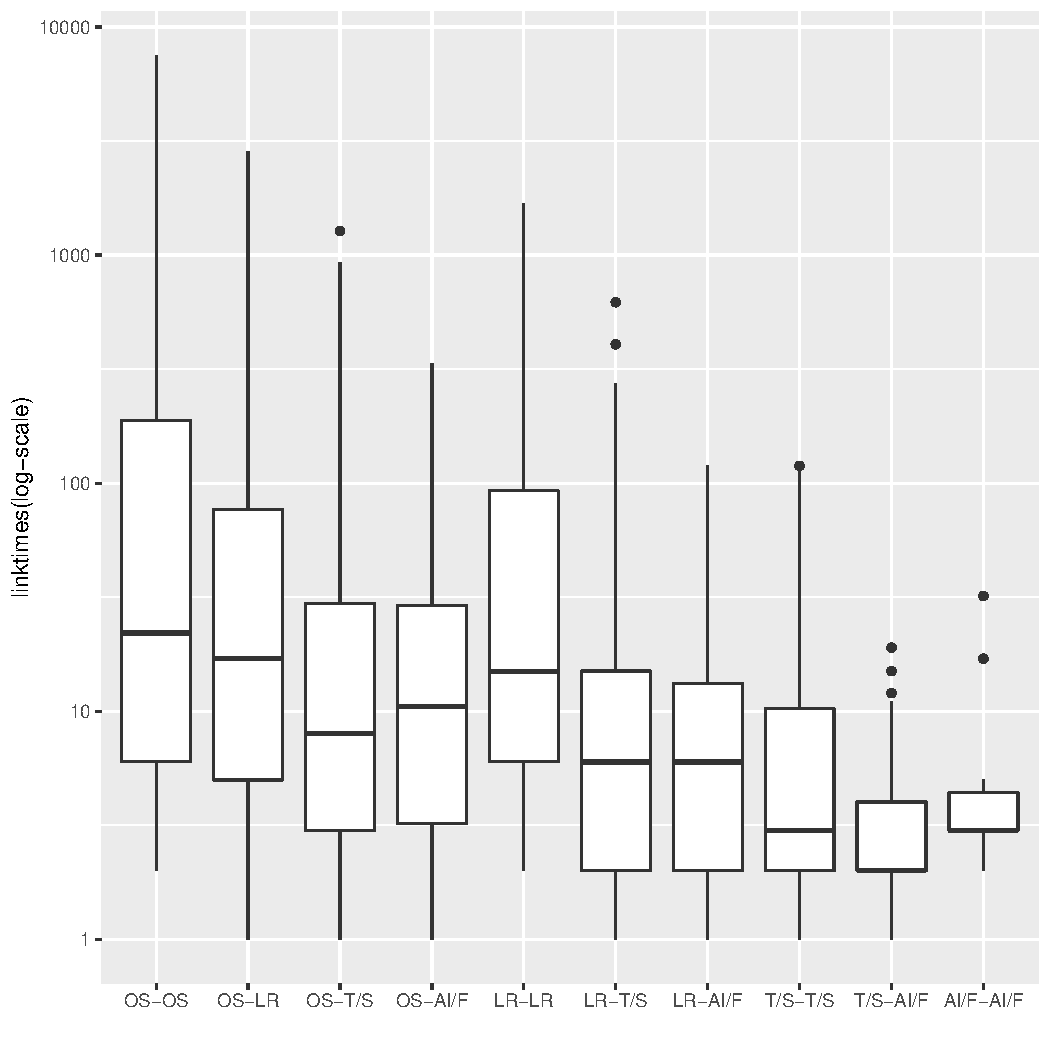
\includegraphics[width=0.5\textwidth]{picture//typepairs_linktimes.pdf}}
\caption{Subimages Net linktimes In Group}
\label{fig}
\end{figure}


Regardless of Other- due to fuzzy features, we statistics and analysis the feature of \emph{linking strength} another 10 kinds of subnetwork pairs  showed as Figure 5. We can get an obvious law of linking realitionships between subnetworks: OS-OS OS-LR LR-LR OS-AI/F     OS-TS are obviously tight linking network pairs while  T/S-AI/F T/S-T/S AI/F AI/F are obviously loose linking network pairs. 

Interestingly, T/S AI/F nearly didn't combain with network tha same type as oneself, however, they are more concerned with subnetworks whose type are OS or LR.   
Because they are inclined to the upper layer of among the whole computer system ...Relatively speaking, OS and LR provide more foundational aids for software development.





Based on the the subnetworks type count in TOP-100 and type feature ranked by linking strength, we consider relatively tight subnetworks pairs including OS-OS OS-LR LR-LR OS-TS and LR-TS OS-AI/F deserve further analysis and explaination. These mode are closely related to software evolution.


\noindent\textbf{OS-OS }  This paradigm can be understood as docker image can be built on several different types of operating systems and run successfully due to the common unix kernel of these distribution operating systems. For instance, even if a image built by centos image can also function as ubuntu kernel running on ubuntu operating system if the applications does not depend on the kernel. The similarity result between operating systems  can be applied to operating systems recommenation when building docker images based on the principle of lightweight. 
 

\noindent\textbf{OS-LR }  In this paradigm, docker image are built based on the basic functions support of system software, such as scheduling tasks, executing applications, and controlling peripherals and meanwhile the support of programming language designed to work on a variety of platforms. Compared with other paradigms, the linking compansess of this paradigm is easiest to understand duo to the foundational aids of these two type images. 

\noindent\textbf{LR-LR }  In this paradigm, docker image are built because of different function modules may be more appropriate to use different languages. {\color{blue} Acturally, Many large-scale software development is not limited to one language. }Interestingly, It often appears that one dockerfile may depend on two basic images at the same time in this paradigm. eg. The front-end development uses php while after-end development uses java. 


\noindent\textbf{OS-TS }  In this paradigm, operating systems manages all of the other application programs in a computer and application/tools make use of the operating system. So the clostest linking to applications is that the operating system is not hard to understand.

%A potential explanation is that 

\noindent\textbf{LR-TS }



\noindent\textbf{OS-AI/F }






\begin{mybox}
OS-OS OS-LR LR-LR OS-AI/F OS-TS are obviously tight linking network pairs while  T/S-AI/F T/S-T/S AI/F AI/F are obviously loose linking network pairs. OS-OS OS-LR LR-LR OS-TS are closely related to software evolution.
\end{mybox}





\section{DISCUSSION}
%Data collected from mobile phones have the potential to provide insight into the underlying 
%Every computer program, web application, and smartphone app has a creative mind behind it.
\subsection{Implication}
\begin{itemize}
\item \textbf{For researchers.}

\noindent\textbf{Automatic Image Summary Generation} Many images stored in Docker Hub, having no tags or function describtion is not conducive to understand or practical usage. 
Our instruction extraction and utilization of dockerfile is conducive to automatic generation image summary.



\noindent\textbf{Image Recommendation} Following the insights from our previous section, we envision a recommender system that analyzes an existing Dockerfile and produces transformations such that the same application can be run with a different base image to reduce the overall size and preferably also build time. 

\noindent\textbf{Recommendation by function description}

\noindent\textbf{Related Image recommendations}We consider two kinds of recommendation applications for docker images. One is to automatically recommend the basic image, which can intelligently help users use the image to build application according to the functional requirements proposed by users, and promote the promotion and use of docker. The other is to recommend the related basic images according to the results of our research on the relationship between core images, especially for those basic images with similar or substitutable functions to reduce the overall size and preferably also build time.


\noindent\textbf{Image Version Techencial debt} Although we neglected the image version to carry out our research, an interesting problem is the technical debt caused by the frequent changes of the image version. If we ignore the two different versions of images with different functions, the quality of image construction may be affected, but how and even to what extent it influences to be further studied, and our research on the difference and relationship between subnetworks is also helpful to address this problem. It is worth mentioning that the recommendation of image version will also help to improve construction quality of image. 




\noindent\textbf{Image Tag recommendations} Image tags can quickly help users to increase their understanding of images, but in dockerhub, most private images are lack of labels, which is not conducive to users' use of them. Our construction of image network and  research of image subnetworks relationship can help the image automatically generate descriptive tags, especially for the newly constructed image. 



\noindent\textbf{Instruction Completion}


\noindent\textbf{Knowledge Graph for}


\item \textbf{For developers.}
\item \textbf{For tool builders.}
\end{itemize}

\subsection{Threats to Validity}
\noindent\textbf{Image Dependency Network Construct}

\noindent\textbf{Linking strength between images}







\section{RELATED WORK}

\subsection{Docker Images Deplyment}

\subsection{Software Ecosystems}






\section{CONCLUSION}
Our method opens the door for future research in docker images ecosystems and knowledge-driven docker images including studying the intelligent recommendation of docker images, the maintaince and repairment of docker images. In this paper, we systematically investigate 






\section*{Acknowledgment}

The preferred spelling of the word ``acknowledgment'' in America is without 
an ``e'' after the ``g''. Avoid the stilted expression ``one of us (R. B. 
G.) thanks $\ldots$''. Instead, try ``R. B. G. thanks$\ldots$''. Put sponsor 
acknowledgments in the unnumbered footnote on the first page.







\section*{References}

Please number citations consecutively within brackets \cite{b1}. The 
sentence punctuation follows the bracket \cite{b2}. Refer simply to the reference 
number, as in \cite{b3}---do not use ``Ref. \cite{b3}'' or ``reference \cite{b3}'' except at 
the beginning of a sentence: ``Reference \cite{b3} was the first $\ldots$''

Number footnotes separately in superscripts. Place the actual footnote at 
the bottom of the column in which it was cited. Do not put footnotes in the 
abstract or reference list. Use letters for table footnotes.

Unless there are six authors or more give all authors' names; do not use 
``et al.''. Papers that have not been published, even if they have been 
submitted for publication, should be cited as ``unpublished'' \cite{b4}. Papers 
that have been accepted for publication should be cited as ``in press'' \cite{b5}. 
Capitalize only the first word in a paper title, except for proper nouns and 
element symbols.

For papers published in translation journals, please give the English 
citation first, followed by the original foreign-language citation \cite{b6}.


\vspace{12pt}
\color{red}
IEEE conference templates contain guidance text for composing and formatting conference papers. Please ensure that all template text is removed from your conference paper prior to submission to the conference. Failure to remove the template text from your paper may result in your paper not being published.


\end{document}
\endinput
%%
%% End of file `sample-sigconf.tex'.
